\label{fs-acker-preliminaries}

\subsection{Overview}

\tracker\ framework bases on another idea of the propagation the fact that the substream ends. Instead of injecting special elements directly into the dataflow, we design a special agent (process) that:

\begin{enumerate}
    \item Receives signals that a substream terminated from data producers.
    \item Watches for in-flight elements and if they belong to some substream.
    \item Notifies dataflow processes when the substream ends {\em for them}, i.e., when they do not receive any elements which satisfy some predicate.
\end{enumerate}

\begin{figure}[htbp]
  \centering
  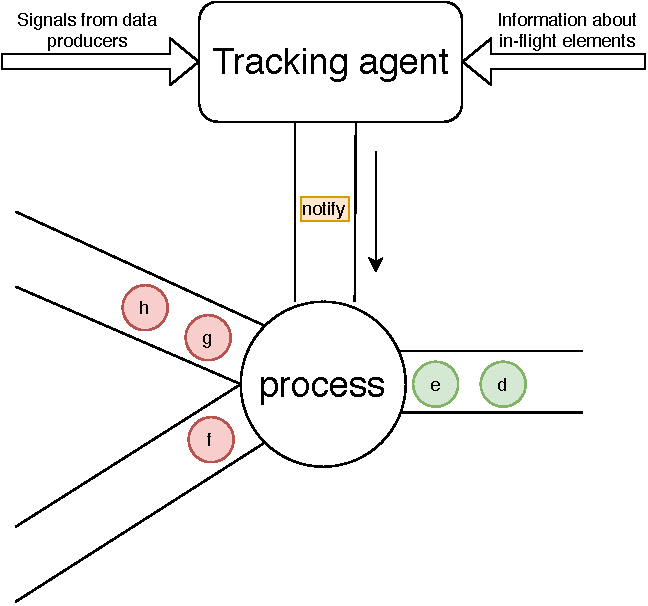
\includegraphics[width=0.35\textwidth]{pics/tracker-scheme.pdf}
  \caption{\tracker\ framework: an example}
  \label{tracker_scheme}
\end{figure}

The general scheme of the \tracker\ mechanism is shown in Figure~\ref{tracker_scheme}. Special (possibly distributed) {\em tracking agent} receives signals from data sources, fetches information about in-flight elements, and then decides to send notifications about substream end. Before diving into implementation details, we should answer the following questions regarding \tracker\ framework, as explained in the next subsection.

{\bf Q1 How to organize monitoring of in-flight elements and to spawn the notifications?} To notify processes that a substream ends, the tracking agent should receive the corresponding signal from data producers and ensure no in-flight elements belong to the substream. 

{\bf Q2 How to provide the consistent notifications order?} Unlike punctuations, \tracker\ notifications are completely async with dataflow elements because they go through another network channel. Hence, dataflow items and notifications are not ordered, making it hard to ensure that notifications order is consistent.

{\bf Q3 What are the functional and performance properties of \tracker?} \tracker\ framework is designed to eliminate the limitations of punctuations framework. We should demonstrate that it is suitable for cyclic dataflows as well as can provide lower network overhead.

\subsection{Discussion}

\subsubsection{Answering Q1: How to organize monitoring of in-flight elements and to spawn the notifications?}
Assume that each process sends to tracking agent the following information about each sending or receiving event $e = <action,m>$:
\begin{enumerate}
    \item $action$: send or receive.
    \item $pred(m)$: the result of applying a substream predicate.
    \item process identifier.
\end{enumerate}

Note that the result of applying predicates can be a vector if we are tracking multiple substreams. Process identifier is an optional field that can be used to send notifications independently for various processes or parts of the physical graph. We will discuss it in detail in the next section.

Using this information along with signals from data producers, the tracking agent can detect when there is a guarantee that a substream ends and send a corresponding notification $e^{n} = <send,pred(m)>$. Therefore, function $S(E_{proc})$ for the \tracker\ framework is the following:

\begin{align*}
& S_{tracker}(E_{proc}) = \exists e^{n} \in E_{proc} : e^{n} = \langle recv,pred(m)\rangle_{tracker,p}
\end{align*}

To make this function satisfy the strict notifications guarantee, one needs to block an input channel if the element that does not belong to the substream arrives. After the notification from \tracker\ arrives, the channel is unblocked. This technique is quite similar to the punctuations alignment, mentioned in the previous section. The processing order function $R_{tracker}(e)$ for this case should satisfy the following condition:

\begin{align*}
& \exists q \in I_p, e = \langle recv,m \rangle_{q,p}: \neg pred(m) \Longrightarrow \\ 
& R_{tracker}(e) > R_{tracker}(e^{n}= \langle recv,pred(m) \rangle_{tracker,p})
\end{align*}

The correctness of the notification guarantees for \tracker\ depends on the implementation of the tracking agent detailed in the next section. The formal proofs that functions $S_{tracker}(E_{proc})$, $R_{tracker}(e)$ along with the \tracker\ implementation satisfy the general and strict guarantees are in the appendix~\ref{appendix:tracker-proof}.

\subsubsection{Answering Q2: How to provide the consistent notifications order?}
To provide a consistent order of notifications, one can define a coincident order between notifications and dataflow items. While in punctuations, such order is provided by design, because punctuations and ordinary data items go through the same FIFO network channels, in \tracker\, this order should be artificially defined.

Assume that SPE assigns to input data elements special totally ordered labels $t(m)$, i.e. $\forall q\in \Pi,a\in A, e=\langle send,m\rangle_{aq}, \exists t(m)$. All data elements which are generated from the input item inherit the label: 

$$\forall q\in \Pi, e=\langle proc,m,M_i\rangle_q, \forall x \in M_i : t(x) = t(m)$$.

In this case, if the order on $t(x)$ coincides with the order of input elements, then \tracker\ can send the notifications according to this order as well. In other words, \tracker\ can reorder its notifications such that they will be consistent with the substreams order. An example of this concept is shown in Figure~\ref{tracker_ordering}. The substream containing element with $t(m)=1$ ends before the substream containing element with $t(m)=2$. As we can see, the order of notifications from \tracker\ coincides with $t(m)$.

\begin{figure}[htbp]
  \centering
  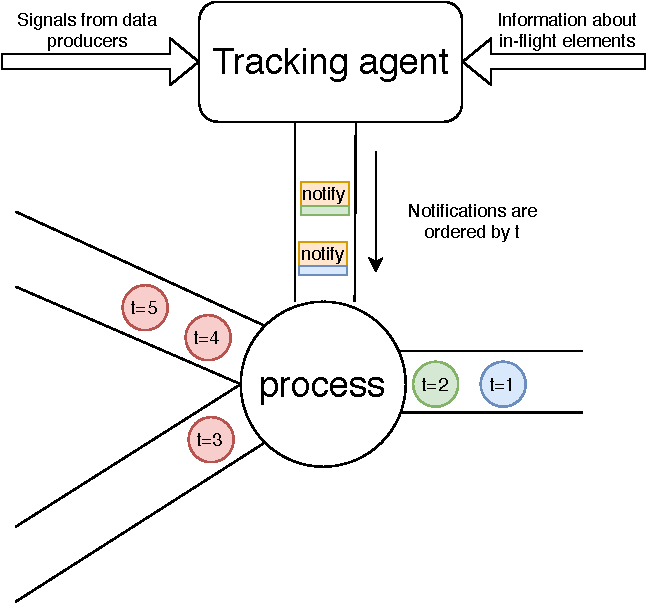
\includegraphics[width=0.35\textwidth]{pics/tracker-ordering.pdf}
  \caption{\tracker\ framework: notifications order}
  \label{tracker_ordering}
\end{figure}

A vital question here is how to implement the assignment of ordered labels $t(m)$. One way is to use the {\em time oracle} service~\cite{???} which can provide totally ordered labels. A simple alternative implementation is detailed in the next section. 

\subsubsection{Answering Q3: What are the functional and performance properties of \tracker?}

The change of the method of the propagation the fact that the substream ends allows \tracker\ to have the following features by design:

\begin{enumerate}
    \item {\bf Cyclic dataflows support.} Because the tracking agent is monitoring for the properties of in-flight elements without direct injection of service items into a dataflow, \tracker\ does not face the problem of throwing them through a cycle.
    \item {\bf Low network overhead.} \tracker\ does not require regular broadcasting of the elements to all computational nodes. As we show in the next section, the amount of service network needed for \tracker\ is $O(D+||\Pi||)$, where $D$ is the depth of a dataflow (logical graph), and $||\Pi||$ is the number of computational nodes (processes). 
\end{enumerate}

At the same time, \tracker\ can provide both general and strict guarantees along with the consistent order of notifications. A limitation of the \tracker\ framework is a potentially more complex implementation than punctuations. The details of the straightforward implementation of the \tracker\ framework are discussed in the next section.
